\chapter{Threats of Browser API Manipulation}
\label{sec.threats}

This chapter investigates the implications of \browserAPI{} manipulation and, through several examples, demonstrates the threats that this can pose. The term “\browserAPI{} manipulation” refers to the modification or overwriting of JavaScript \acsp{api} provided by the browser engine. While manipulation of \acsp{api} is not inherently malicious, as explained in the fundamentals \autoref{sec.browserAPIs} and \autoref{sec.polyfill} about Browser APIs and Polyfills, this chapter only addresses the malicious use-cases. First, \autoref{sec.threatmodel} presents the threat model that this investigation is based on. Then, the following sections describe potential threats, with each section focusing on a specific group of \acsp{api} that share similar properties and implications. An overview of these threats can be seen in \autoref{tab.threats}.

\begin{table}[h]
    \parbox{\linewidth}{
    \centering
    \begin{tabularx}{\textwidth}{l|p{30mm}|p{45mm}|X}
        Section & Affected APIs & Threats & Implications \\
        \hline
        \ref{sec.threats.requestinterception} &
        \minline{fetch}, \minline{XMLHttpRequest} &
        Interception and manipulation of network requests that originate from scripts &
        Compromises data integrity by allowing manipulation of data being sent and received;
        Can be used for application layer \acs{ddos}~attacks
        \\\hline
        \ref{sec.threats.crypto.plaintext} &
        \minline{crypto.subtle} &
        Access to plain-text data before it is encrypted &
        Compromises data confidentiality by allowing access to and exfiltration of unencrypted data
        \\\hline
        \ref{sec.threats.entropy} &
        \minline{crypto} &
        Manipulation of pseudo random numbers &
        Compromises security of passwords, tokens and cryptographic keys generated based on random numbers
        \\\hline
        \ref{sec.threats.intercept-privileged} &
        privileged APIs such as Geolocation or Web Authentication &
        Intercept requests to sensitive data and credentials &
        Compromises the confidentiality of sensitive data; Stolen credentials can be used for impersonation
    \end{tabularx}
    \caption{Summary of threats presented in this chapter}
    \label{tab.threats}
    }
\end{table}



\section{Threat Model}
\label{sec.threatmodel}

This section presents the threat model that the investigation of threats is based on. Contrary to conventional threat models (cf. \cite{ChromiumSecArchitecture}), which generally have the goal of developing countermeasures against threats, this threat model assumes that web applications are vulnerable in order to assess the resulting threats. The primary goal of this thesis is to \textit{detect} the threats, which will be discussed in \autoref{sec.detection}. In the first part of this section, we will take a look at the roles and components of the threat model and visualize how they interact with each other. Then, potential entry points for code execution are presented and finally, the attackers' goals are defined, as well as their abilities and limitations.

The considered threat model includes the following main components: the user, browser, browser extensions, web servers and web application code. \autoref{fig.threat-model-components} shows the relationship and interactions between these components. The user interacts with the browser, e.g. visits a website and interacts with dialogs. The browser communicates with web servers over the internet, which are responsible for relaying the web application code. Web applications consist of first party code and can also include code from third-parties. This can either be done directly, when the third-party code is hosted on the first party web server, or by indirectly including the code from third-party servers such as a \ac{cdn}. Third-party servers can also be used to deliver first party code.

\begin{figure}[H]
    \centering
    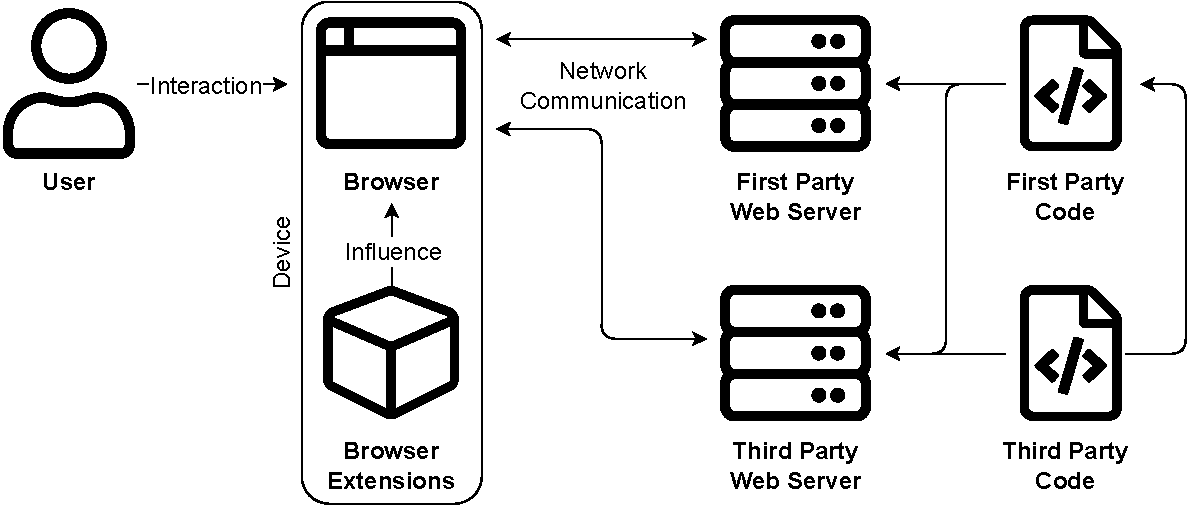
\includegraphics[width=13.9cm]{img/threat-model.pdf}
    \caption{Components of the Threat Model}
    \label{fig.threat-model-components}
\end{figure}

\BrowserAPIs{} are accessible through the \hyperref[sec.globals]{global \icode{window} object} and can be overwritten the same way as any other variable (cf. \autoref{sec.browserAPIs}). As the window object is not shared across different web pages, an attacker needs to be able to execute JavaScript code in the context of the targeted web page in order to manipulate \browserAPIs{}. This can be achieved in the following cases:

\begin{enumerate}
    \item If security vulnerabilities are present in a web application that allow an attacker to execute code in the users browser, such as \ac{xss} vulnerabilities.
    \item Through \ac{mitm} attacks that intercept the communication between the browser and web servers, allowing the injection of arbitrary code. This is possible when the connection is insecure, e.g. when \acs{http} is used instead of \acs{https}.
    \item If the attacker is able to modify third-party code that is included in the web application. This could, for example, be an open-source library that the attacker has control over.
    \item When the attacker is able to control a third-party web server that hosts code included in the web application.
    \item If the browser is running an extension that is controlled by the attacker and has the required privileges to inject code into web pages.
\end{enumerate}

The attacker can visit websites and analyze them for security vulnerabilities and JavaScript inclusions. The analysis may reveal possible points of entry as listed above. If an attacker detects the usage of third-party JavaScript code in a web application, they can attempt to modify the official distribution source, either where the code is downloaded from or where it is remotely included from. If the third-party JavaScript code originates from an open-source project, the attacker could attempt to contribute malicious code to it, in order for it to eventually be distributed. The attacker can also analyze the dependency chains of remote inclusions as well as the dependency chains of libraries that the web application uses. This can reveal additional entry points that can be compromised.

The execution of JavaScript code allows an attacker to control a web application and access associated data such as cookies and the local storage. Here, we will only focus on the threats posed by \browserAPI{} manipulation and not the usage of \browserAPIs{}.

There are, however, some restrictions to the constructed attacker. The attacker is not able to access data from other web applications. Due to the browser security architecture described in \autoref{sec.browser-security-architecture} and the same origin policy explained in \autoref{sec.origin}, it is generally not possible for an attacker to access data of other web pages. The browser security architecture also makes it impossible for the web application to access the filesystem unless users explicitly choose and grant access to a file themselves.

The attacker considered in this threat model has at least one of the following goals:

\begin{enumerate}
    \item Impersonate users through a web application. This includes performing actions as the targeted user inside of the web application and signing or encrypting data as the user.
    \item Manipulate the behavior of web applications and the users actions. This can, for example, include modifying the information that is sent and displayed to the user or modifying the data that the user sends to the web application.
    \item Access private data from users that is controlled by the web application. This includes cryptographic keys and plaintext before it is encrypted.
    \item Cause a denial of service of the web application.
\end{enumerate}



\section{Network Request Interception and Manipulation}
\label{sec.threats.requestinterception}

\minline{Fetch} and \minline{XMLHttpRequest} are \browserAPIs{} that allow sending \acs{http} requests. Overwriting them would give an attacker control over the data being sent and received by a web application. This is effectively a \ac{mitm} attack limited to network requests originating from JavaScript code and allows an attacker to intercept and manipulate users actions and data, thereby compromising data integrity. This also allows attackers to cause a client-side \ac{dos} which can be used to target specific users and prevent them from using the web application or even specific functionality of the application.

Furthermore, attackers can use these \acsp{api} for an application layer \ac{ddos}~attack by amplifying the amount of requests generated by users. Unlike traditional \ac{ddos}~attacks, which target the network layer using techniques such as \acs{udp} or \acs{tcp}~SNY flooding, application layer \ac{ddos}~attacks are designed to flood the web application with legitimate requests that are computationally expensive to process. For attackers, this has the benefit of being more effective at overloading the targeted systems and harder to mitigate due to requests being indistinguishable from ones generated by legitimate users. \cite{ApplicationLayerDDoS}

As an example of request manipulation, let us take a look at a hypothetical banking web application that allows transferring money to a recipient, which is implemented by sending transaction data encoded as \acs{json} to a \acs{rest}~\acs{api} reachable at \minline{/api/transfer-money}. To send the data, the web application uses the \minline{fetch}~\acs{api}, as shown in listing \ref{lst.fetchExample}. If an attacker were to inject code that changes the behavior of \minline{fetch}, such that it would examine and change data before being sent, it would be possible to change the behavior of the web application without needing to change the specific code of the application that is responsible for processing user input and sending the data.

\begin{lstlisting}[language=JavaScript,label={lst.fetchExample},caption={Fetch request with \acs{json} data}]
fetch("/api/transfer-money", {
    method: "POST",
    body: JSON.stringify({
        recipient: "Alice"
    })
});
\end{lstlisting}

Listing \ref{lst.fetchManipulation} shows code that, when injected, stores a reference to the original \minline{fetch}~\acs{api} and then overwrites \minline{fetch} with code that replaces the recipient in the \acs{json} data passed to it with \minline{"Eve"} and then sends the modified request using the original \minline{fetch}~\acs{api}. This would result in all transactions now being sent to Eve, instead of Alice.

\begin{lstlisting}[language=JavaScript,label={lst.fetchManipulation},caption={Overwriting fetch to manipulate data under certain conditions}]
// Store original fetch
const originalFetch = window.fetch;

// Overwrite fetch
window.fetch = (resource, init) => {
    // Only change request under certain conditions
    if (resource === "/api/transfer-money") {
        if (typeof init?.body === "string") {
            let data = JSON.parse(init.body)
            data.recipient = "Eve";
            init.body = JSON.stringify(data);
        }
    }
    // Send request via original fetch API
    return originalFetch(resource, init);
};
\end{lstlisting}



\section{Cryptography Backdoors}
\label{sec.threats.crypto}

The Web Cryptography \acs{api} provides an interface for web applications to generate and store cryptographic keys, which can be used to encrypt, decrypt, sign and verify data. The interfaces can be accessed through the globally accessible \icode{crypto} and \icode{crypto.subtle} objects. While the objects themselves are defined to be read-only, their methods can be modified, which allows changing their behavior. \cite{crypto}

Most of these \acs{api} methods, with the exception of \icode{crypto.getRandomValues()}, are only available in a secure context, such as pages loaded over \acs{https} \cite{crypto}. This prevents the use of functions intended to handle sensitive data in an insecure context, as this could otherwise make it possible for attackers to inject code or manipulate data using a \ac{mitm} attack.



\subsection{Data Exfiltration}
\label{sec.threats.crypto.plaintext}

An attacker could modify the \icode{crypto.subtle.encrypt} method such that data is exfiltrated before it is encrypted. An example of this is shown in \autoref{lst.encrypt-middleware}, where first, a reference to the original method is stored and then the method is overwritten to decode and log the plaintext. Finally, the arguments are passed along to the original method and its result is returned. Instead of logging the text, it could also be exfiltrated using the fetch \acs{api} to send the data to a webserver controlled by the attacker. It would also be possible to first store the data locally and exfiltrate it at a later time to obfuscate the malicious behavior and reduce the chance of detection.

\begin{lstlisting}[language=JavaScript,label={lst.encrypt-middleware},caption={Interception of data before it is encrypted}]
// store reference to original function
let origEncrypt = crypto.subtle.encrypt;

// overwrite the API
crypto.subtle.encrypt = (algorithm, key, data) => {
    // access the plaintext before it is encrypted
    let decoder = new TextDecoder();
    let plaintext = decoder.decode(data);
    console.log("Plaintext:", plaintext);

    // call the original function and return the encrypted data
    return origEncrypt.apply(crypto.subtle, [algorithm, key, data]);
};
\end{lstlisting}



\subsection{Entropy Manipulation}
\label{sec.threats.entropy}

Another method of the Web Cryptography \acs{api} is \icode{crypto.getRandomValues()}, which takes a typed array as an argument, e.g. a \icode{Uint8Array} or \icode{Int32Array}, and overwrites all elements of the provided array with cryptographically strong random values matching its type \cite{crypto}. The specification states that implementations should seed the \ac{prng} with a good source of entropy, such as the source provided by the \ac{os}, but does not contain any requirements to the level of entropy guaranteed by the \acs{api}. While this method should not be used to generate cryptographic keys, it can be used to generate random tokens, passwords or any other sequence that is required to be random.

It is possible to overwrite \icode{getRandomValues()} and thereby compromise the integrity of any code that depends on the entropy of its result. An attacker could replace the method with a function that returns a known sequence instead of a random one, as shown in \autoref{lst.random-fixed-value} where the provided array is filled with the fixed value \icode{4}.

\begin{lstlisting}[language=JavaScript,escapeinside={/*!}{!*/},escapebegin=\itshape\color{magenta!90!black},label={lst.random-fixed-value},caption={Returning fixed instead of random values.}]
crypto.getRandomValues = array => {
    array.fill(4); // /*!\href{https://xkcd.com/221/}{chosen by fair dice roll.}!*/
                   // /*!\href{https://xkcd.com/221/}{guaranteed to be random.}!*/
    return array;
};
\end{lstlisting}
% https://xkcd.com/221/
% https://dilbert.com/strip/2001-10-25

A more sophisticated attack could provide a polyfill that generates seemingly random values while actually choosing values that follow a pattern known to the attacker. This could also be achieved using a \ac{prng} with a known seed or a predictable seed with a low quality of entropy.



\section{Intercepting Privileged APIs}
\label{sec.threats.intercept-privileged}

\BrowserAPIs{} that allow web applications to request access to sensitive information, such as Geolocation, require users to give their consent by confirming a dialog that prompts them for permission. In order for an attacker to use these \acsp{api}, they would need to get users to confirm such a dialog. This requires attackers to convince users of two things: first, that the website needs the data that is being requested and second, that the website is trustworthy. Traditional approaches such as phishing might not be able to convince users of these statements. If an attacker is able to overwrite these \browserAPIs{} on a web application that the user already trusts, they can simply wait for the web application to request the permission to access the sensitive information and intercept the response once access has been granted. The response can be intercepted by storing a reference to the \ac{api} function and overwriting the browser \ac{api} with a new function that acts as an intermediary by calling the reference of the original \ac{api} and exfiltrating the response data.

Another \ac{api} that is relevant to the goals of the attacker is the Web Authentication \ac{api}, which is used to securely authenticate a user through a web application \cite{webauthn}. One of the security features of the \ac{api} is that it prevents phishing sites from stealing credentials by binding the credentials to the origin of a site \cite{webauthn}. Intercepting calls from a web application to this \ac{api} would allow attackers to steal the credentials associated with the site and use them to gain access to the users account and impersonate them.
